\hypertarget{day-11---ux7f16ux5199ux65e5ux5fd7ux521bux5efaux9875}{%
\subsection{Day 11 -
编写日志创建页}\label{day-11---ux7f16ux5199ux65e5ux5fd7ux521bux5efaux9875}}

在 Web 开发中,后端代码写起来其实是相当容易的。

例如,我们编写一个 REST API,用于创建一个 Blog:

\begin{pythoncode}
@post('/api/blogs')
def api_create_blog(request, *, name, summary, content):
    check_admin(request)
    if not name or not name.strip():
        raise APIValueError('name', 'name cannot be empty.')
    if not summary or not summary.strip():
        raise APIValueError('summary', 'summary cannot be empty.')
    if not content or not content.strip():
        raise APIValueError('content', 'content cannot be empty.')
    blog = Blog(user_id=request.__user__.id, user_name=request.__user__.name, user_image=request.__user__.image, name=name.strip(), summary=summary.strip(), content=content.strip())
    yield from blog.save()
    return blog
\end{pythoncode}

编写后端 Python 代码不但很简单,而且非常容易测试,上面的
API:\texttt{api\_create\_blog()}本身只是一个普通函数。

Web 开发真正困难的地方在于编写前端页面。前端页面需要混合 HTML、CSS 和
JavaScript,如果对这三者没有深入地掌握,编写的前端页面将很快难以维护。

更大的问题在于,前端页面通常是动态页面,也就是说,前端页面往往是由后端代码生成的。

生成前端页面最早的方式是拼接字符串:

\begin{pythoncode}
s = '<html><head><title>'
    + title
    + '</title></head><body>'
    + body
    + '</body></html>'
\end{pythoncode}

显然这种方式完全不具备可维护性。所以有第二种模板方式:

\begin{pythoncode}
<html>
<head>
    <title>{{ title }}</title>
</head>
<body>
    {{ body }}
</body>
</html>
\end{pythoncode}

ASP、JSP、PHP 等都是用这种模板方式生成前端页面。

如果在页面上大量使用
JavaScript(事实上大部分页面都会),模板方式仍然会导致 JavaScript
代码与后端代码绑得非常紧密,以至于难以维护。其根本原因在于负责显示的
HTML DOM 模型与负责数据和交互的 JavaScript 代码没有分割清楚。

要编写可维护的前端代码绝非易事。和后端结合的 MVC
模式已经无法满足复杂页面逻辑的需要了,所以,新的
\href{http://en.wikipedia.org/wiki/Model_View_ViewModel}{MVVM}:Model
View ViewModel 模式应运而生。

MVVM 最早由微软提出来,它借鉴了桌面应用程序的 MVC 思想,在前端页面中,把
Model 用纯 JavaScript 对象表示:

\begin{pythoncode}
<script>
    var blog = {
        name: 'hello',
        summary: 'this is summary',
        content: 'this is content...'
    };
</script>
\end{pythoncode}

View 是纯 HTML:

\begin{pythoncode}
<form action="/api/blogs" method="post">
    <input >
    <input >
    <textarea ></textarea>
    <button type="submit">OK</button>
</form>
\end{pythoncode}

由于 Model 表示数据,View 负责显示,两者做到了最大限度的分离。

把 Model 和 View 关联起来的就是 ViewModel。ViewModel 负责把 Model
的数据同步到 View 显示出来,还负责把 View 的修改同步回 Model。

ViewModel 如何编写?需要用 JavaScript 编写一个通用的
ViewModel,这样,就可以复用整个 MVVM 模型了。

好消息是已有许多成熟的 MVVM 框架,例如 AngularJS,KnockoutJS
等。我们选择 \href{http://vuejs.org/}{Vue} 这个简单易用的 MVVM
框架来实现创建 Blog 的页面\texttt{templates/manage\_blog\_edit.html}:

\begin{pythoncode}


编辑日志



<script>
var
    ID = '{{ id }}',
    action = '{{ action }}';
function initVM(blog) {
    var vm = new Vue({
        el: '#vm',
        data: blog,
        methods: {
            submit: function (event) {
                event.preventDefault();
                var $form = $('#vm').find('form');
                $form.postJSON(action, this.$data, function (err, r) {
                    if (err) {
                        $form.showFormError(err);
                    }
                    else {
                        return location.assign('/api/blogs/' + r.id);
                    }
                });
            }
        }
    });
    $('#vm').show();
}
$(function () {
    if (ID) {
        getJSON('/api/blogs/' + ID, function (err, blog) {
            if (err) {
                return fatal(err);
            }
            $('#loading').hide();
            initVM(blog);
        });
    }
    else {
        $('#loading').hide();
        initVM({
            name: '',
            summary: '',
            content: ''
        });
    }
});
</script>





    <div class="uk-width-1-1 uk-margin-bottom">
        <div class="uk-panel uk-panel-box">
            <ul class="uk-breadcrumb">
                <li><a href="/manage/comments">评论</a></li>
                <li><a href="/manage/blogs">日志</a></li>
                <li><a href="/manage/users">用户</a></li>
            </ul>
        </div>
    </div>

    <div id="error" class="uk-width-1-1">
    </div>

    <div id="loading" class="uk-width-1-1 uk-text-center">
        <span><i class="uk-icon-spinner uk-icon-medium uk-icon-spin"></i> 正在加载...</span>
    </div>

    <div id="vm" class="uk-width-2-3">
        <form v-on="submit: submit" class="uk-form uk-form-stacked">
            <div class="uk-alert uk-alert-danger uk-hidden"></div>
            <div class="uk-form-row">
                <label class="uk-form-label">标题:</label>
                <div class="uk-form-controls">
                    <input v-model="name" >
                </div>
            </div>
            <div class="uk-form-row">
                <label class="uk-form-label">摘要:</label>
                <div class="uk-form-controls">
                    <textarea v-model="summary" rows="4" ></textarea>
                </div>
            </div>
            <div class="uk-form-row">
                <label class="uk-form-label">内容:</label>
                <div class="uk-form-controls">
                    <textarea v-model="content" rows="16" ></textarea>
                </div>
            </div>
            <div class="uk-form-row">
                <button type="submit" class="uk-button uk-button-primary"><i class="uk-icon-save"></i> 保存</button>
                <a href="/manage/blogs" class="uk-button"><i class="uk-icon-times"></i> 取消</a>
            </div>
        </form>
    </div>


\end{pythoncode}

初始化 Vue 时,我们指定 3 个参数:

el:根据选择器查找绑定的 View,这里是\texttt{\#vm},就是 id
为\texttt{vm}的
DOM,对应的是一个\texttt{\textless{}div\textgreater{}}标签;

data:JavaScript 对象表示的
Model,我们初始化为\texttt{\{\ name:\ \textquotesingle{}\textquotesingle{},\ summary:\ \textquotesingle{}\textquotesingle{},\ content:\ \textquotesingle{}\textquotesingle{}\}};

methods:View 可以触发的 JavaScript
函数,\texttt{submit}就是提交表单时触发的函数。

接下来,我们在\texttt{\textless{}form\textgreater{}}标签中,用几个简单的\texttt{v-model},就可以让
Vue 把 Model 和 View 关联起来:

\begin{pythoncode}
<input v-model="name" class="uk-width-1-1">
\end{pythoncode}

Form
表单通过\texttt{\textless{}form\ v-on="submit:\ submit"\textgreater{}}把提交表单的事件关联到\texttt{submit}方法。

需要特别注意的是,在 MVVM 中,Model 和 View 是双向绑定的。如果我们在
Form 中修改了文本框的值,可以在 Model
中立刻拿到新的值。试试在表单中输入文本,然后在 Chrome 浏览器中打开
JavaScript
控制台,可以通过\texttt{vm.name}访问单个属性,或者通过\texttt{vm.\$data}访问整个
Model:

 
 \begin{figure}[htp]
	\centering
	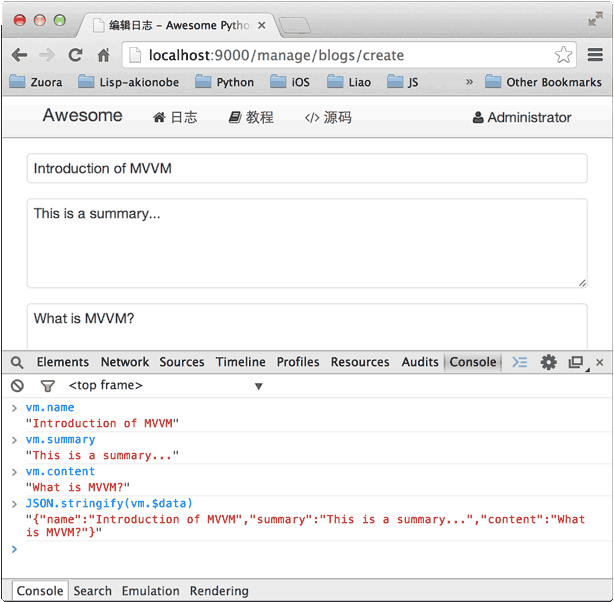
\includegraphics[width=0.6\linewidth]{fig/956056345770752.png}
\end{figure}


如果我们在 JavaScript 逻辑中修改了 Model,这个修改会立刻反映到 View
上。试试在 JavaScript
控制台输入\texttt{vm.name\ =\ \textquotesingle{}MVVM简介\textquotesingle{}},可以看到文本框的内容自动被同步了:

 
 \begin{figure}[htp]
	\centering
	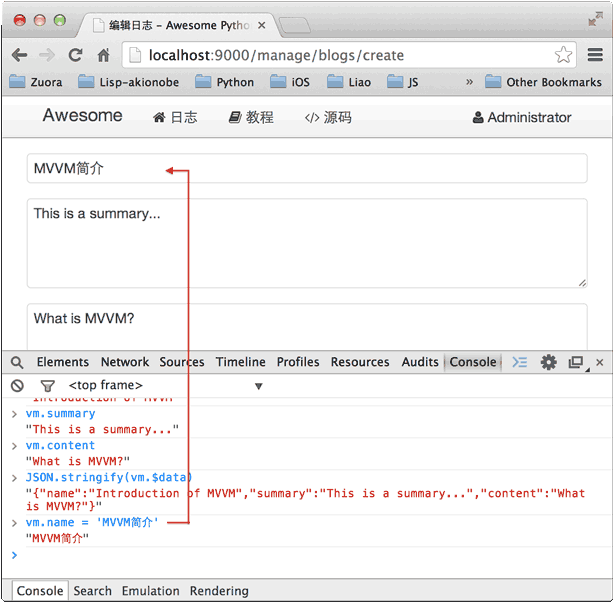
\includegraphics[width=0.6\linewidth]{fig/956056362546592.png}
\end{figure}


双向绑定是 MVVM 框架最大的作用。借助于
MVVM,我们把复杂的显示逻辑交给框架完成。由于后端编写了独立的 REST
API,所以,前端用 AJAX 提交表单非常容易,前后端分离得非常彻底。

\hypertarget{ux53c2ux8003ux6e90ux7801}{%
\subsubsection{参考源码}\label{ux53c2ux8003ux6e90ux7801}}

\href{https://github.com/michaelliao/awesome-python3-webapp/tree/day-11}{day-11}

